\section{收缩和不动点}
\label{section:ch09-sec55}

我们现在来运用 $S^{1}$ 的基本群的知识证明拓扑学的几个经典结论.

\begin{definition}[收缩与收缩核]
\label{definition:ch09-sec55-retraction}
若 $A\subset X$, 一个连续映射 $r\colon X\to A$ 如果在 $A$ 上的限制是 $A$ 上的恒等映射, 则称之为 $X$ 到 $A$ 上的一个\textbf{收缩}(retraction). 如果存在这样一个收缩 $r$, 则说 $A$ 是 $X$ 的一个\textbf{收缩核}(retract).
\end{definition}

\begin{lemma}
\label{lemma:ch09-sec55-55-1}
如果 $A$ 是 $X$ 的收缩核, 那么内射 $j\colon A\to X$ 诱导的基本群的同态是一个单射.
\end{lemma}

\begin{proof}
如果 $r\colon X\to A$ 是一个收缩, 则复合映射 $r\circ j$ 等于 $A$ 上的恒等映射. 这蕴涵着 $r_*\circ j_*$ 是 $\pi_1(A,a)$ 的恒等映射, 因此 $j_*$ 是单射.
\end{proof}

\begin{theorem}[非收缩定理]
\label{theorem:ch09-sec55-55-2}
从 $B^{2}$ 到 $S^{1}$ 上没有收缩.
\end{theorem}

\begin{proof}
如果 $S^{1}$ 是 $B^{2}$ 的一个收缩核, 则内射 $j\colon S^{1}\to B^{2}$ 的诱导同态是一个单射. 但 $S^{1}$ 的基本群不是平凡群而 $B^{2}$ 的基本群是平凡群. 这是一个矛盾.
\end{proof}

\begin{lemma}
\label{lemma:ch09-sec55-55-3}
设 $h\colon S^{1}\to X$ 是连续映射. 则以下条件等价:
\begin{enumerate}
\item $h$ 是零伦的.
\item $h$ 可以扩张为一个连续映射 $k\colon B^{2}\to X$.
\item $h_*$ 是基本群间的平凡同态.
\end{enumerate}
\end{lemma}


\begin{proof}
(1)$\Rightarrow$(2). 设 $H\colon S^{1}\times I\to X$ 是 $h$ 与某一个常值映射之间的同伦. 设 $\pi\colon S^{1}\times I\to B^{2}$ 为映射, 定义为
\[
\pi(x,t)=(1-t)x.
\]
$\pi$ 是连续的、闭的、满的, 因而是一个商映射, 它将 $S^{1}\times 1$ 收缩成为点 $\boldsymbol{0}$, 而在其他地方是单的. 由于 $H$ 在 $S^{1}\times 1$ 上取常值, 它通过商映射 $\pi$ 诱导出一个连续映射 $k\colon B^{2}\to X$, $k$ 是 $h$ 的扩张. 参见图 \cref{figure:ch09-fig-55-1}.


(2)$\Rightarrow$(3). 设 $j\colon S^{1}\to B^{2}$ 是内射, 则 $h$ 等于复合 $k\circ j$. 因此 $h_*=k_*\circ j_*$. 然而, 由于 $B^{2}$ 的基本群是平凡的, 所以
\[
j_{*}\colon\pi_{1}(S^{1},b_{0})\longrightarrow\pi_{1}(B^{2},b_{0})
\]
是平凡的. 因此 $h_*$ 是平凡的.

(3)$\Rightarrow$(1). 设 $p\colon\mathbb{R}\to S^{1}$ 是标准的覆叠映射, $p_0\colon I\to S^{1}$ 为其在单位区间上的限制, 则 $[p_0]$ 是 $\pi_1(S^{1},b_0)$ 的一个生成元, 因为 $p_0$ 是 $S^{1}$ 中的回路, 它开始于 $0$ 的提升在 $1$ 处终结.

设 $x_0=h(b_0)$. 由于 $h_*$ 是平凡的, 回路 $f=h\circ p_0$ 代表 $\pi_1(X,x_0)$ 的单位元. 因此, $X$ 中 $f$ 与 $x_0$ 处的常值道路之间有一个道路同伦 $F$. 由于映射 $p_0\times\mathrm{id}\colon I\times I\to S^{1}\times I$ 是连续的、闭的、满的, 所以它是一个商映射. 对于每一个 $t$, $p_0\times\mathrm{id}$ 将 $0\times t$ 和 $1\times t$ 都映为 $b_0\times t$, 而在其他地方是单的. 道路同伦 $F$ 将 $0\times I$、$1\times I$ 和 $I\times 1$ 映到 $X$ 的点 $x_0$, 所以它诱导出一个连续映射 $H\colon S^{1}\times I\to X$, 这个连续映射是 $h$ 和某一个常值映射之间的同伦. 参见图 \cref{figure:ch09-fig-55-2}.
\end{proof}


\begin{corollary}
\label{corollary:ch09-sec55-55-4}
内射 $j\colon S^{1}\to\mathbb{R}^{2}-\boldsymbol{0}$ 不是零伦的. 恒等映射 $i\colon S^{1}\to S^{1}$ 也不是零伦的.
\end{corollary}

\begin{proof}
有一个从 $\mathbb{R}^{2}-\boldsymbol{0}$ 到 $S^{1}$ 的收缩, 其定义为 $r(x)=x/\|x\|$. 因此, $j_*$ 是单射, 因而是非平凡的. 类似地, $i_*$ 是恒等同态, 因而也是非平凡的.
\end{proof}

\begin{theorem}
\label{theorem:ch09-sec55-55-5}
对于任意给定的 $B^{2}$ 上的一个非蜕化向量场, 存在 $S^{1}$ 中的一个点, 这个点上的向量直指内向, 也存在 $S^{1}$ 中的一个点, 这个点上的向量直指外向.
\end{theorem}

\begin{proof}
$B^{2}$ 上的一个\textbf{向量场}(vector field) 是一个有序偶 $(x,v(x))$, 其中 $x\in B^{2}$, $v$ 是从 $B^{2}$ 到 $\mathbb{R}^{2}$ 中的一个连续映射. 在微积分中, 常用记号
\[
\boldsymbol{v}(x)=v_{1}(x)\boldsymbol{i}+v_{2}(x)\boldsymbol{j}
\]
代替函数 $v$, 其中 $\boldsymbol{i}$, $\boldsymbol{j}$ 是 $\mathbb{R}^{2}$ 中的标准单位基向量, 而我们还是使用简单的函数记号. 一个向量场称为\textbf{非蜕化的}, 如果对于所有 $x$, $v(x)\neq\boldsymbol{0}$, 这时, 自然将 $B^{2}$ 映到 $\mathbb{R}^{2}-\boldsymbol{0}$ 中.

先假设 $v(x)$ 在 $S^{1}$ 的任何点 $x$ 上都不是直指内向的, 然后导出矛盾. 考虑映射 $v\colon B^{2}\to\mathbb{R}^{2}-\boldsymbol{0}$. 设 $w$ 是 $v$ 在 $S^{1}$ 上的限制. 由于映射 $w$ 有一个扩充将 $B^{2}$ 映到 $\mathbb{R}^{2}-\boldsymbol{0}$ 之中, 所以它是零伦的.

另一方面, $w$ 同伦于内射 $j\colon S^{1}\to\mathbb{R}^{2}-\boldsymbol{0}$. 图 \cref{figure:ch09-fig-55-3} 诠释了这个同伦, 我们用方程给出形式的定义如下: 对于 $x\in S^{1}$,
\[
F(x,t)=tx+(1-t)w(x).
\]
我们应当指出 $F(x,t)\neq\boldsymbol{0}$. 明显地, 当 $t=0$ 或 $t=1$ 时, $F(x,t)\neq\boldsymbol{0}$. 如果对于某一个 $t$, $0<t<1$, 有 $F(x,t)=\boldsymbol{0}$, 则 $tx+(1-t)w(x)=\boldsymbol{0}$. 因此 $w(x)$ 等于 $x$ 与某一个负数的乘积, 而这意味着 $w(x)$ 在点 $x$ 上直指内向! 因此 $F$ 的确是一个从 $S^{1}\times I$ 到 $\mathbb{R}^{2}-\boldsymbol{0}$ 的映射.

这推出 $j$ 是零伦的, 与前一推论矛盾.

为了证明 $v$ 在 $S^{1}$ 的某一个点上直指外向, 只需将刚才证明的结论应用于向量场 $(x,-v(x))$ 就可以了.
\end{proof}


我们已经知道每一个连续映射 $f\colon[0,1]\to[0,1]$ 必定有一个不动点 (参见第 24 节中的习题 3). 其实对于球 $B^{2}$ 而言同样的结论也成立, 然而证明却更为深刻.

\begin{theorem}[圆盘的 Brouwer 不动点定理]
\label{theorem:ch09-sec55-55-6}
如果 $f\colon B^{2}\to B^{2}$ 是连续的, 则存在一个点 $x\in B^{2}$ 使得 $f(x)=x$.
\end{theorem}

\begin{proof}
我们用反证法来证明. 设对于 $B^{2}$ 中的每一个 $x$, $f(x)\neq x$. 定义 $v(x)=f(x)-x$, 我们便得到了 $B^{2}$ 上的一个非蜕化的向量场 $(x,v(x))$. 然而向量场 $v$ 在 $S^{1}$ 上没有一个点 $x$ 直指外向, 因为这意味着对于某一个正实数 $a$,
\[
f(x)-x=ax,
\]
于是 $f(x)=x+ax$ 将处于单位球 $B^{2}$ 的外面. 这是一个矛盾.
\end{proof}

在数学中不动点定理令人感兴趣的原因在于许多问题 (例如, 方程组的解的存在性问题) 都能化为不动点问题. 这里给出一个例子, 即经典的 Frobenius 定理. 假设读者已经具备了线性代数的一些知识.

\begin{corollary}
\label{corollary:ch09-sec55-55-7}
设 $A$ 是一个 $3\times 3$ 的正实数矩阵, 则 $A$ 有一个正的实特征值.
\end{corollary}

\begin{proof}
设 $T\colon\mathbb{R}^{3}\to\mathbb{R}^{3}$ 是一个线性变换, 其 (相对于 $\mathbb{R}^{3}$ 的标准基而言的) 矩阵为 $A$. 又设 $B$ 为二维球面 $S^{2}$ 与 $\mathbb{R}^{3}$ 的第一卦限
\[
\{\,(x_{1},x_{2},x_{3})\mid x_{1}\geqslant 0,\ x_{2}\geqslant 0,\ x_{3}\geqslant 0\,\}
\]
的交. 不难证明, $B$ 同胚于球体 $B^{2}$, 所以对于 $B$ 到自身的连续映射, 不动点定理成立.

若 $x=(x_1,x_2,x_3)\in B$, 则 $x$ 的所有分量都是非负的, 并且至少有一个分量是正的. 由于 $A$ 的所有元素都是正的, 所以向量 $T(x)$ 的所有分量都是正的. 因此, 映射 $x\mapsto T(x)/\|T(x)\|$ 为 $B$ 到自身的一个连续映射, 从而有一个不动点 $x_0$. 于是
\[
T(x_{0})=\|T(x_{0})\|\,x_{0},
\]
所以 $T$ (从而矩阵 $A$) 有一个正的实特征值 $\|T(x_0)\|$.
\end{proof}

最后, 我们证明一个定理. 这个定理蕴涵着 $\mathbb{R}^{2}$ 中的三角形区域
\[
T=\{\,(x,y)\mid x\geqslant 0,\ y\geqslant 0\text{ 并且 }x+y\leqslant 1\,\}
\]
的拓扑维数至少是 $2$. (参见第 50 节.)

\begin{theorem}
\label{theorem:ch09-sec55-55-8}
存在 $\varepsilon>0$ 使得对于任何一个由直径小于 $\varepsilon$ 的集合组成的 $T$ 的开覆盖 $\mathcal{A}$, $T$ 中总有某一个点至少属于 $\mathcal{A}$ 的三个元素之中.
\end{theorem}

\begin{proof}
由于 $T$ 同胚于 $B^{2}$, 因此可以将本节中证明的结论应用于空间 $T$.

选取 $\varepsilon>0$ 使得没有一个直径小于 $\varepsilon$ 的集合和 $T$ 的所有三条边都相交. (事实上, $\varepsilon=\frac{1}{2}$ 就可以.) 我们假设 $\mathcal{A}=\{U_1,\cdots,U_n\}$ 是 $T$ 的一个开覆盖, 其中每一个 $U_i$ 的直径都小于 $\varepsilon$, 使得 $\mathcal{A}$ 中任何三个元素都无交, 然后由此导出矛盾.

对于每一个 $i=1,\cdots,n$, 选取 $T$ 的一个顶点 $v_i$ 如下: 如果 $U_i$ 与 $T$ 的两条边相交, 令 $v_i$ 为这两条边的公共顶点. 如果 $U_i$ 只与 $T$ 的一条边相交, 令 $v_i$ 为这条边的端点中的一个. 如果 $U_i$ 与 $T$ 的任何一条边都无交, 令 $v_i$ 为 $T$ 的任意顶点.

现设 $\{\phi_i\}$ 是由 $\{U_1,\cdots,U_n\}$ 控制的单位分拆. (参见第 36 节.) 定义 $k\colon T\to\mathbb{R}^{2}$ 如下:
\[
k(x)=\sum_{i=1}^{n}\phi_{i}(x)v_{i}.
\]
则 $k$ 是连续的. 给定 $T$ 中的一个点 $x$, 它最多属于 $\mathcal{A}$ 的两个元素, 因此最多只有两个 $\phi_i(x)$ 是
非零的. 所以, 如果 $x$ 仅属于一个开集 $U_i$, 则存在 $0\leqslant t\leqslant 1$, 使得 $k(x)=v_i$; 如果 $x$ 属于两个开集 $U_i$ 和 $U_j$, 则 $k(x)=tv_i+(1-t)v_j$. 无论何种情形, $k(x)$ 都属于 $T$ 的三条边的并 $\mathrm{Bd}\,T$ 中. 于是 $k$ 将 $T$ 映到 $\mathrm{Bd}\,T$ 中.

此外, $k$ 将 $T$ 的每一条边映到自身. 因为如果 $x$ 属于 $T$ 的边 $vw$, 任意包含 $x$ 的开集 $U_i$ 都要与这条边相交, 因此 $v_i$ 必然等于 $v$ 或 $w$. 由 $k$ 的定义可见 $k(x)$ 属于 $vw$.

设 $h\colon\mathrm{Bd}\,T\to\mathrm{Bd}\,T$ 为 $k$ 在 $\mathrm{Bd}\,T$ 上的限制. 因为 $h$ 能够被扩充为连续映射 $k$, 所以它是零伦的. 另一方面, $h$ 同伦于 $\mathrm{Bd}\,T$ 到自身的恒等映射. 因为 $h$ 将每一条边映到自身, $h$ 与 $\mathrm{Bd}\,T$ 的恒等映射之间的直线同伦便是所需的同伦. 然而, $\mathrm{Bd}\,T$ 的恒等映射 $i$ 绝不是零伦的.
\end{proof}

\subsection*{习题}

\begin{exercise}
证明: 如果 $A$ 是 $B^{2}$ 的一个收缩核, 则每一个连续映射 $f\colon A\to A$ 必有一个不动点.
\end{exercise}

\begin{exercise}
证明: 如果 $h\colon S^{1}\to S^{1}$ 是零伦的, 则 $h$ 必有一个不动点, 并且 $h$ 还将某一个点 $x$ 映为它的对径点 $-x$.
\end{exercise}

\begin{exercise}
证明: 如果 $A$ 是非奇异的 $3\times 3$ 非负矩阵, 则 $A$ 必有一个正的实特征值.
\end{exercise}

\begin{exercise}
假定你已经知道: 对于每一个 $n$, 没有收缩 $r\colon B^{n+1}\to S^{n}$. (这个结论可以用代数拓扑中更为深刻的工具来证明.) 证明以下结论:
\begin{enumerate}
\item 恒等映射 $i\colon S^{n}\to S^{n}$ 不是零伦的.
\item 内射 $j\colon S^{n}\to\mathbb{R}^{n+1}-\boldsymbol{0}$ 不是零伦的.
\item $B^{n+1}$ 上每一个非蜕化向量场必定在 $S^{n}$ 的某一点处直指内向, 也在 $S^{n}$ 的某一点处直指外向.
\item 每一个连续映射 $f\colon B^{n+1}\to B^{n+1}$ 必定有一个不动点.
\item 每一个由正实数组成的 $(n+1)\times(n+1)$ 矩阵必有正的特征根.
\item 如果 $h\colon S^{n}\to S^{n}$ 是零伦的, 则 $h$ 必有一个不动点, 同时 $h$ 也必将某一个点 $x$ 映为它的对径点 $-x$.
\end{enumerate}
\end{exercise}

\begin{figure}[h]
\centering
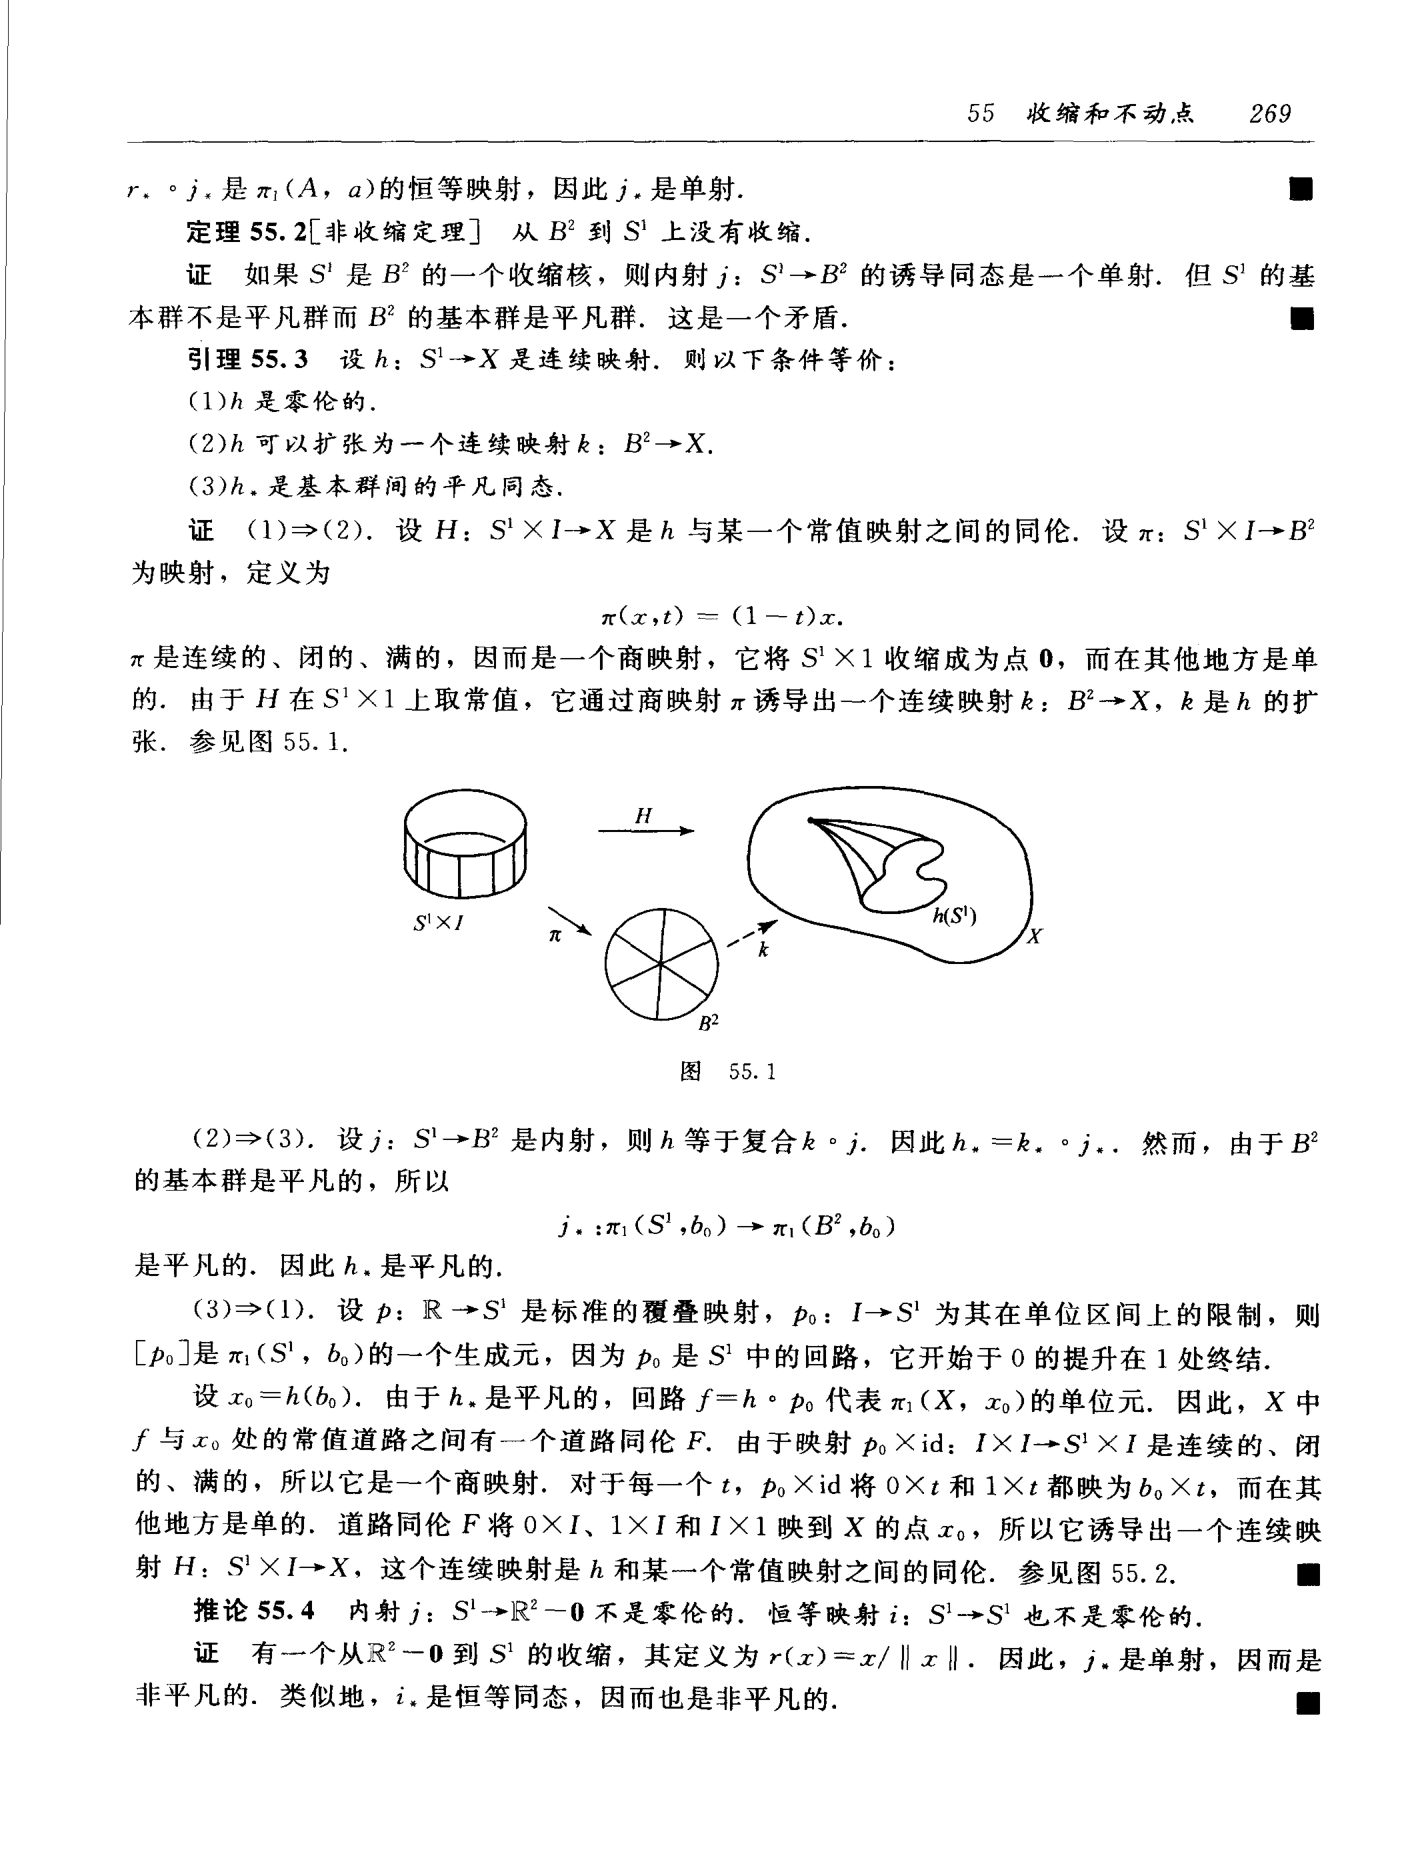
\includegraphics[width=0.6\textwidth]{image/fig-55-1.png}
\caption{引理的证明：(1)$\Rightarrow$(2) 的商映射构造.}
\label{figure:ch09-fig-55-1}
\end{figure}

\begin{figure}[h]
\centering
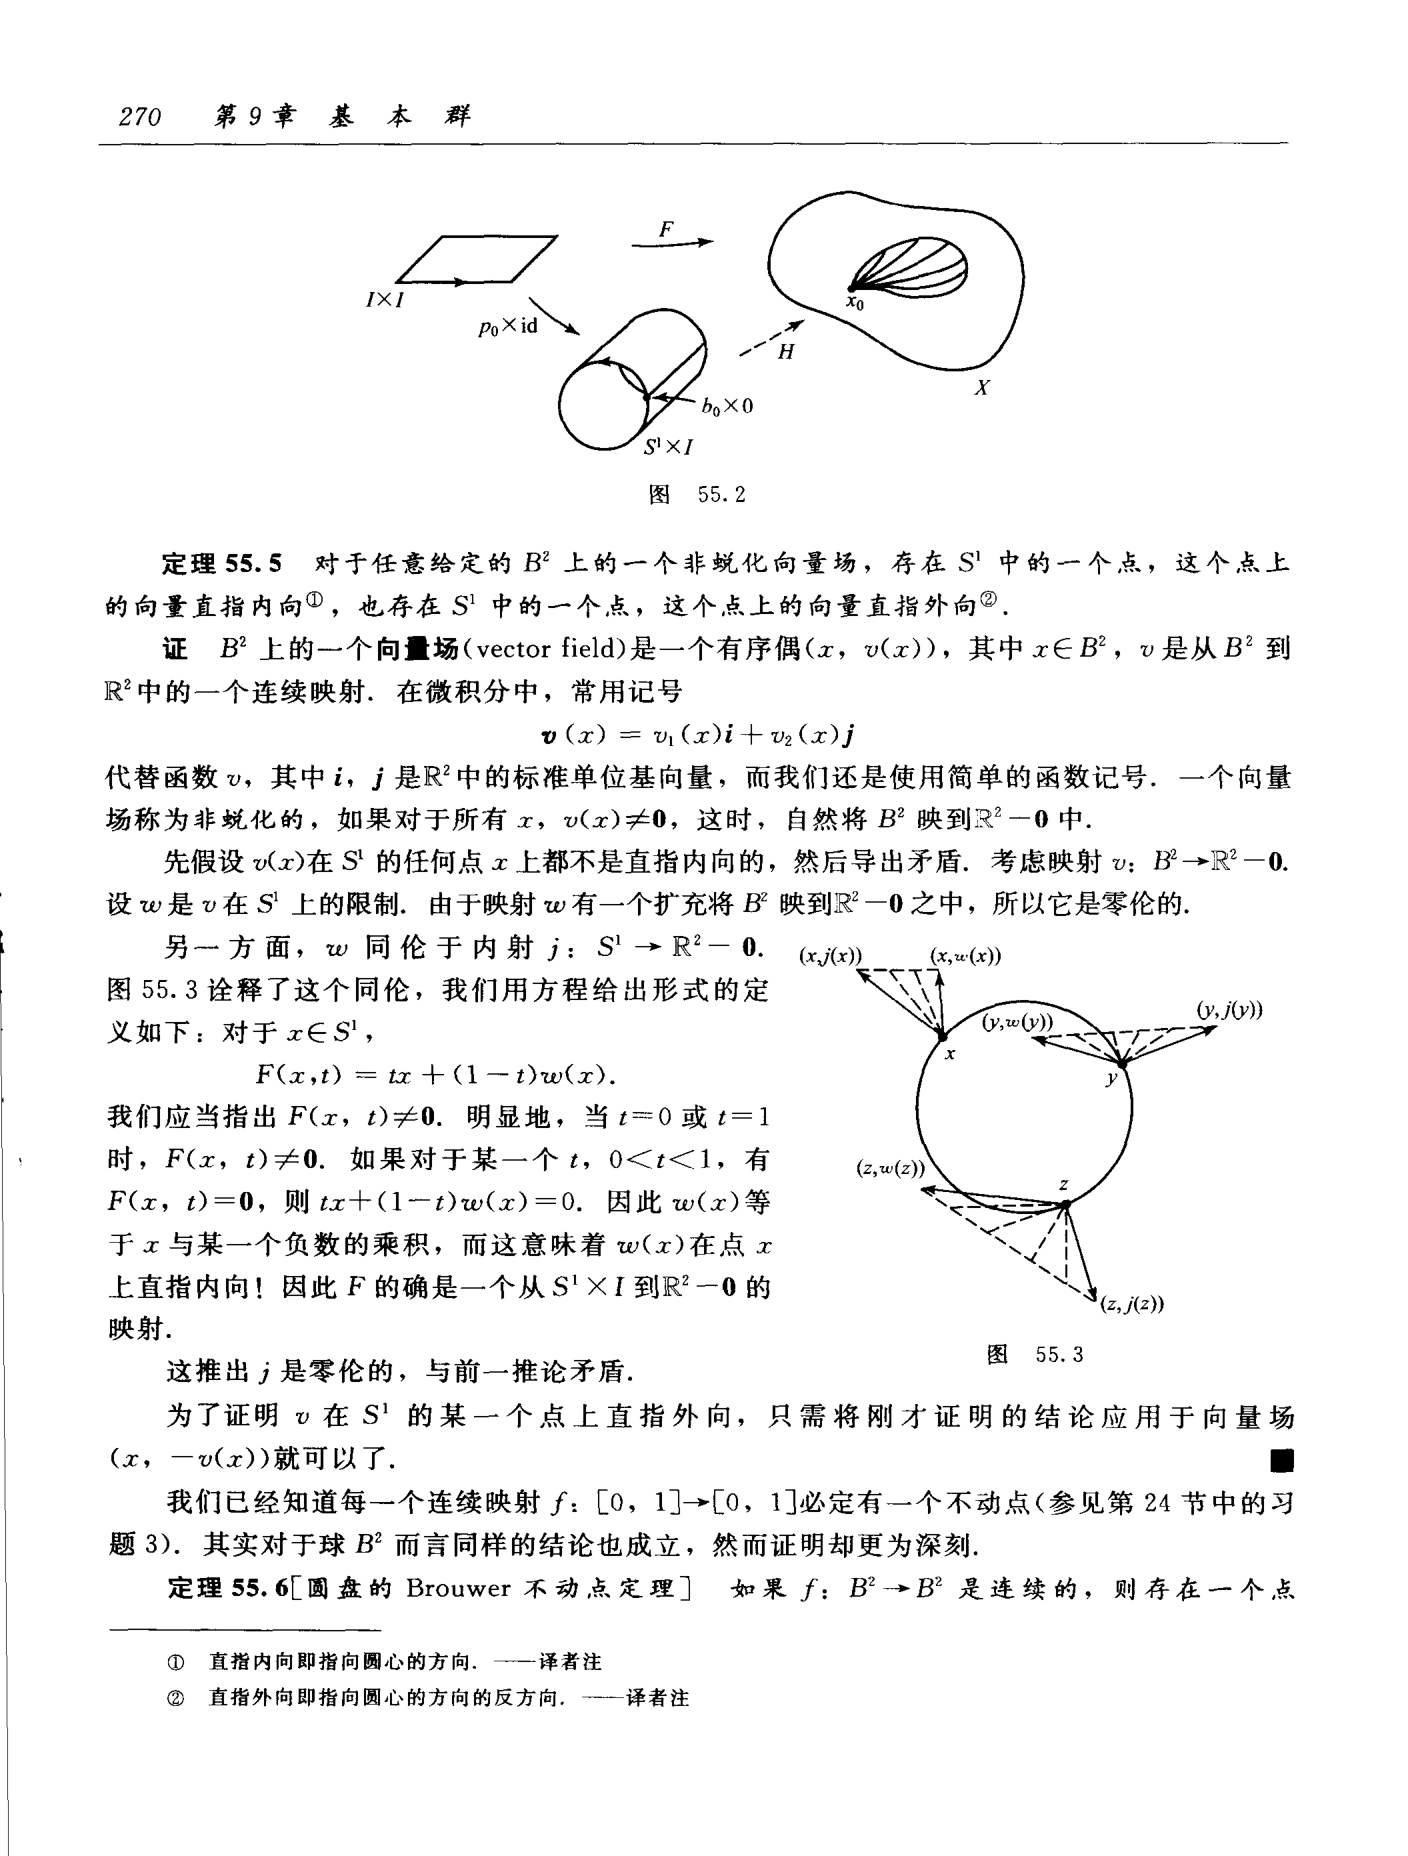
\includegraphics[width=0.6\textwidth]{image/fig-55-2.png}
\caption{引理的证明：(3)$\Rightarrow$(1) 的道路同伦构造.}
\label{figure:ch09-fig-55-2}
\end{figure}

\begin{figure}[h]
\centering
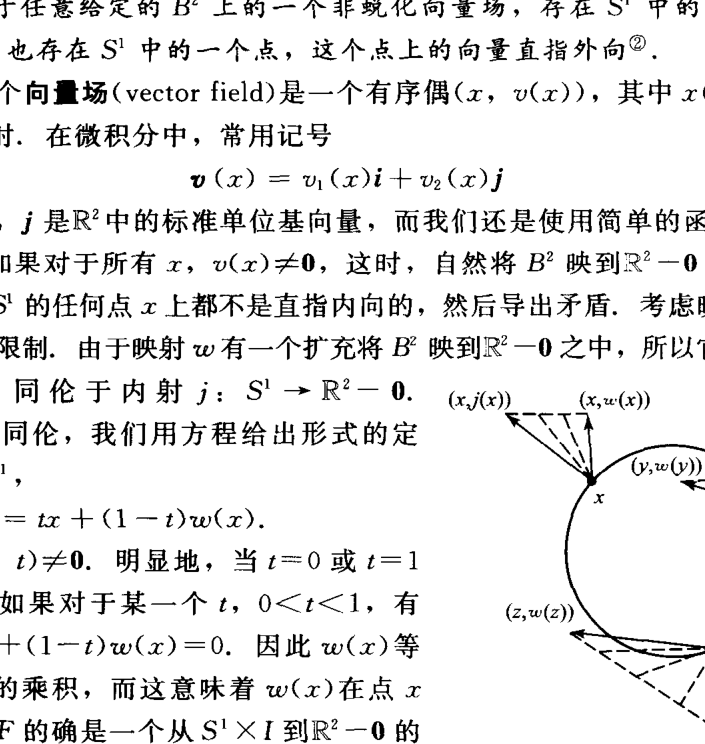
\includegraphics[width=0.6\textwidth]{image/fig-55-3.png}
\caption{向量场 $w$ 同伦于内射 $j$ 的直线同伦 $F(x,t)=tx+(1-t)w(x)$.}
\label{figure:ch09-fig-55-3}
\end{figure}